\section{Architecture globale}
    \label{sec:archiGlobale}
    
    Afin de mieux fixer les idées quant aux fonctionnalités de Glasir, voici une présentation rapide de son utilisation puis de son interface.
	    
    \subsection{Diagramme de cas d'utilisation}
    \label{sec:casutil}
    
    L'utilisateur type de notre outil d'analyse serait un expert en sécurité connaissant déjà le formalisme des ADTrees. C'est donc l'acteur qui a été choisi pour le diagramme de cas d'utilisation de la {\sc Figure}~\ref{fig:use_case}, qui représente l'ensemble des actions possibles à partir de Glasir. Afin de mieux comprendre ce diagramme, un petit rappel sur le formalisme UML s'impose. En effet, les deux termes \og étendre \fg{} et \og inclure \fg{} associés aux différentes flèches ont une signification bien particulière (attention au sens des flèches) :

    \begin{itemize}
    \item A -- \og inclure \fg{} --> B signifie que si A est réalisé, B l'est {\bf forcément} ;
    \item B -- \og étendre \fg{} --> A signifie que si A est réalisé, B {\bf peut} l'être.
    \end{itemize}

    \begin{figure}[H]
        \centering
        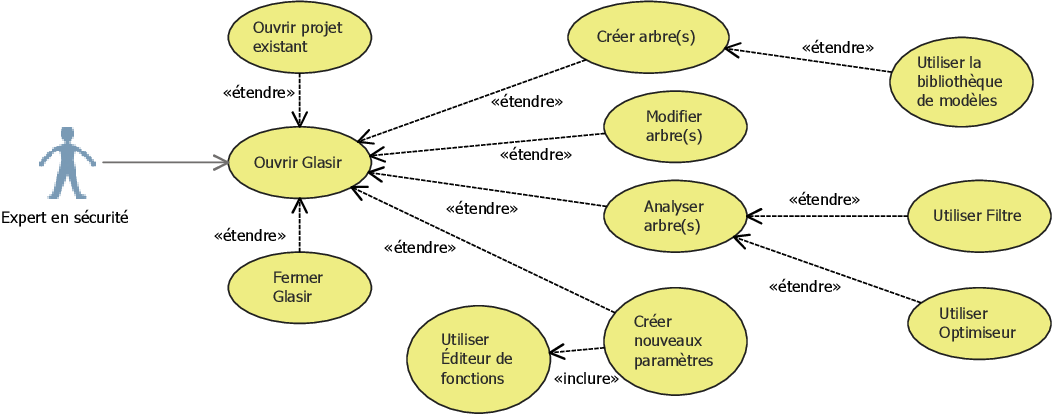
\includegraphics[height=0.5\textwidth]{figure/UseCaseDiagram.png}
        \caption{Diagramme de cas d'utilisation de Glasir.}
        \label{fig:use_case}
    \end{figure}

    Les fonctionnalités de Glasir apparaissent donc maintenant clairement : grâce à lui, l'utilisateur pourra effectuer les actions suivantes : 

    \begin{itemize}
    \item charger un projet sauvegardé ;
    \item créer de nouveaux ADTrees, en utilisant ou non la bibliothèque de modèles ;
    \item modifier des ADTrees déjà existants ;
    \item analyser les ADTrees du projet en cours, à la main ou à l'aide du Filtre ou de l'Optimiseur ;
    \item créer de nouveaux paramètres pour ADTool par le biais de l'Éditeur de fonctions.
    \end{itemize}  

    Toutes ces possibilités seront accessibles facilement grâce à une interface utilisateur claire et fonctionnelle, dont un prototype est présenté à la {\sc Section}~\ref{sec:interface}.      
    
    \subsection{Prototype d'interface}
    \label{sec:interface}
    
    Voici un prototype de l'interface.
    \begin{figure}[h!]
        \centering
        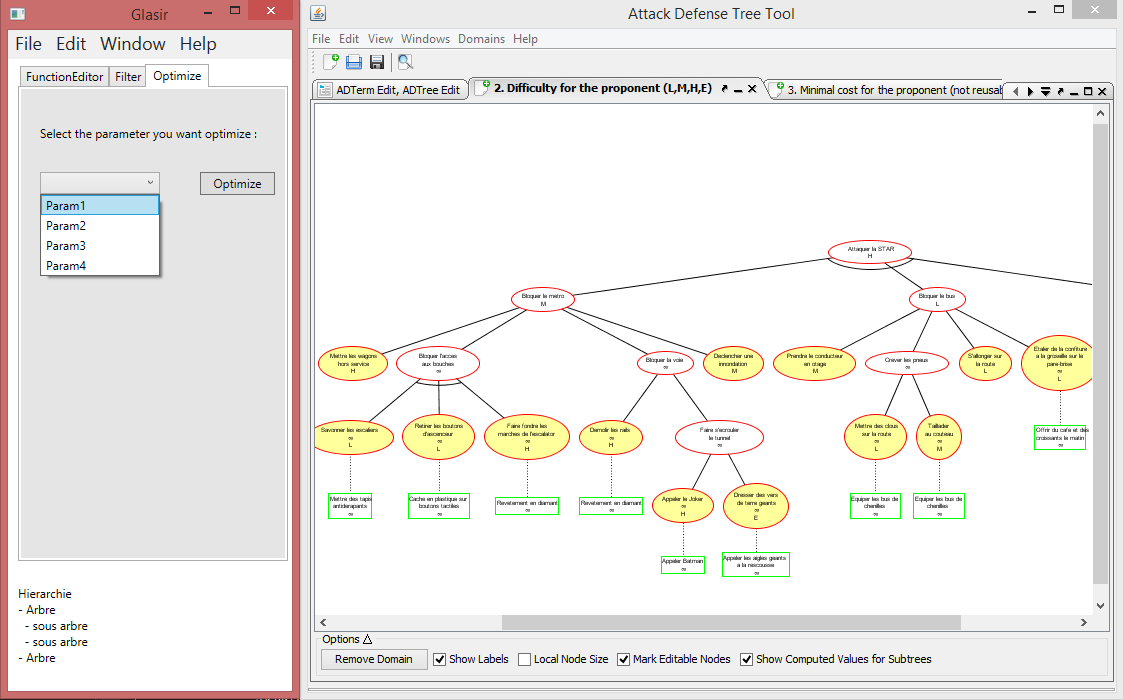
\includegraphics[height=0.4\textwidth]{figure/interface.png}
        \caption{Prototype de l'interface de Glasir.}
        \label{fig:interface}
    \end{figure}
    
    Les fonctions filtre et tout seront facilement accessibles. On aura adtool au milieu ou pas, blablabla.
